\section{Circular Motion}

\subsection{angular quantities}

position vector $\vec{r}$ $\longrightarrow$ angular displacement $\theta$

rate of change in angular displacement $\longrightarrow$ angular velocity: $\boxed{\omega = \ddt{\theta} = \dot{\theta}}$

rate of change in angular velocity $\longrightarrow$ angular acceleration: $\boxed{\alpha = \ddt{\omega} = \ddot{\theta}}$

\subsubsection*{relation to linear quantites}

distance moved out along an arc: $s=\theta r$

linear speed: $v=\ddt{s} = \ddt{(\theta r)} = \ddt{\theta} r \RA \boxed{v=\omega r}$

acceleration is a more complicated issue, we leave that for next subsection

\subsubsection*{uniform accelerated motion}

for uniformly accelerated circular motion, $\alpha = \text{const}$

angular displacement and angular velocity change with time

these are analogous to linear quantities (displacement, velocity, acceleration)

\begin{center}
	\begin{tabular}{|c|c|}
		\hline
		 uniformly accelerated linear motion & uniformly accelerated circular motion \\
		 \hline
		 $v = v_0 + a t$ & $\omega = \omega_0 + \alpha t$\\
		 $s = s_0 + v_0 t + \frac{1}{2}at^2$ & $\theta = \theta_0 + \omega_0 t + \frac{1}{2}\alpha t^2$ \\
		 $2a\Delta s = v^2 - v_0^2$	 &  $2\alpha \Delta \theta = \omega ^2 - \omega_0^2$ \\
		 \hline
	\end{tabular}
\end{center}

\subsection{acceleration}

acceleration is rate of change in velocity, which has both magnitude and direction

for linear motion, only magnitude of velocity changes, so only concept of linear acceleration

for circular motion, both magnitude and direction of velocity can change

we need two types of acceleration, responsible for changing magnitude and direction of $\vec{v}$


\begin{figure}[htp]
	\centering
\begin{minipage}{0.4\textwidth}
\begin{center}
	\begin{tikzpicture}[scale = 1.35]
	\draw[dashed] (0,0) node[below]{$O$} -- (60:5) node[below]{$A$};
	\draw[dashed] (0,0) -- (75:5) node[below left]{$B$};
	\draw[dashed] (50:5) arc(50:85:5);
	\draw[blue,thick,->] (60:5) -- ++(150:1) node[midway, above]{$\vec{v}$};
	\draw[blue,thick,->] (75:5) -- ++(165:1.8) node[midway, above]{$\vec{v}'$};
	\draw (60:1.5) arc(60:75:1.5);
	\node at (68:1.8) {$\Delta \theta$};
	\end{tikzpicture}
\end{center}
\end{minipage}\hfil
\begin{minipage}{0.4\textwidth}
	\begin{center}
		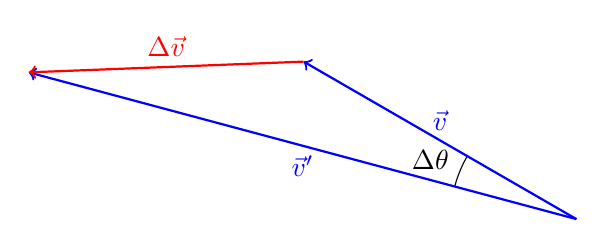
\begin{tikzpicture}[scale=4]
		\draw (150:0.4) arc(150:165:0.4);
		\node at (158:0.5) {$\Delta \theta$};
		\draw[blue,thick,->] (0:0) -- (150:1) node[midway, above]{$\vec{v}$};
		\draw[blue,thick,->] (0:0) -- (165:1.8) node[midway, below]{$\vec{v}'$};
		\draw[->,thick,red] (150:1) -- (165:1.8) node[midway, above]{$\Delta \vec{v}$};
		\end{tikzpicture}
	\end{center}

\centering
$\Downarrow$

	\begin{center}
	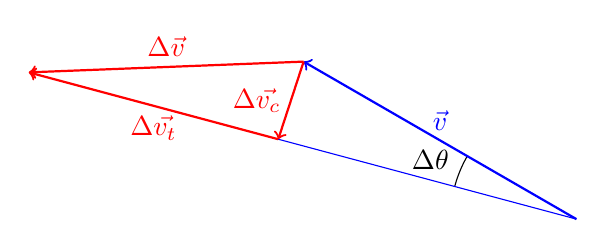
\begin{tikzpicture}[scale=4]
	\draw (150:0.4) arc(150:165:0.4);
	\node at (158:0.5) {$\Delta \theta$};
	\draw[blue,thick,->] (0:0) -- (150:1) node[midway, above]{$\vec{v}$};
	\draw[blue] (0:0) -- (165:0.98);
	\draw[->,thick,red] (150:1) -- (165:1.8) node[midway, above]{$\Delta \vec{v}$};
	\draw[->,thick,red] (150:1) -- (165:0.98) node[midway, left]{$\Delta \vec{v_c}$};
	\draw[->,thick,red] (165:0.98) -- (165:1.8) node[midway, below]{$\Delta \vec{v_t}$};
	\end{tikzpicture}
\end{center}
\end{minipage}
\end{figure}

suppose an object moves from $A$ to $B$ in short time interval $\Delta t$

change in velocity is: $\Delta \vec{v} = \vec{v}' - \vec{v}$

its acceleration: $\vec{a} = \frac{\Delta \vec{v}}{\Delta t} = \frac{\Delta \vec{v_t}}{\Delta t} + \frac{\Delta \vec{v_c}}{\Delta t}$ (see vector diagram)

as $\Delta t \to 0$, $\Delta \theta \to 0$, $\Delta \vec{v_t}$ becomes parallel to $\vec{v}$, $\Delta \vec{v_c}$ becomes normal to $\vec{v}$

so $\Delta \vec{v_t}$ gives an increase in magnitude of velocity, while $\Delta \vec{v_c}$ changes the direction

acceleration can be considered as the sum of two parts: $\boxed{\vec{a} = \vec{a_t} + \vec{a_c}}$

tangential acceleration $a_t$ (or transverse acceleration), that changes magnitude of $\vec{v}$

centripetal acceleration $a_c$ (or normal acceleration), that changes direction of $\vec{v}$

\subsubsection*{tangential acceleration}

from previous discussions, $\boxed{a_t = \ddt{v}}$

$a_t$ is closely related to angular acceleration $\alpha$: $\ddt{v} = \ddt{(\omega r)} = \ddt{\omega} r \RA \boxed{a_t = \alpha r}$ or $\boxed{a_t = \ddot{\theta} r}$

\subsubsection*{centripetal acceleration}

from vector diagram, $\Delta v_c \approx v \Delta \theta$, so $a_c = \frac{\Delta v_c}{\Delta t} \approx \frac{v \Delta \theta}{\Delta t}$

taking the limit $\Delta t \to 0$, $\omega = \ddt\theta$, so $a_c = v\omega$ $\RA$ $\boxed{a_c = \frac{v^2}{r}}$ or $\boxed{ a_c = \omega^2 r  = \dot{\theta}^2 r}$

\subsubsection*{resultant acceleration}

resultant acceleration: $\vec{a} = \vec{a_t} + \vec{a_c}$

where its magnitude is given by: $a = \sqrt{a_t^2 + a_c^2}$

\subsubsection*{vector analysis ($\star$)}

we can formally define $\vec{\omega}$ in terms of a cross product: $\boxed{\vec{v} = \vec{\omega} \times \vec{r}}$

direction of cross product is defined using the right-hand grip rule

\begin{figure}[htp]
	\centering
	\begin{tikzpicture}[scale=1.2]
	\draw (0,0) ellipse (3 and 1);
	\draw (-3,0) -- (-3,-0.1) (3,0) -- (3,-0.1);
	\draw[purple,thick,->] (0,0) node[right]{$O$} --++ (0,2.2) node[left]{$\vec{\omega}$};
	\draw[thick,->] (0,0) -- (159.54:2.134) node[above,midway]{$\vec{r}$};
	\draw[thick,->,blue] (159.54:2.134) -- ++ (200:2) node[above]{$\vec{v}$};
%	\draw[->] (0,0) --++ (-3,-2) node[left]{$x$};
%	\draw[->] (0,0) --++ (4.5,0) node[above]{$y$};
%	\draw[thick, ->] (0.16,1.5) arc(-70:250:0.45 and 0.2);
%	\draw[thick, ->] (4,0.16) arc(20:340:0.2 and 0.45);
%	\draw[thick, ->] (-2.4,-1.8) arc(-100:210:0.4 and 0.25);
	\end{tikzpicture}
\end{figure}

$\vec{a} = \ddt{\vec{v}} = \ddt{(\vec{\omega} \times \vec{r})} = \ddt{\vec{\omega}} \times \vec{r} + \vec{\omega} \times \ddt{\vec{r}} \RA \vec{a} = \vec{\alpha}\times\vec{r} + \vec{\omega}\times(\vec{\omega}\times\vec{r})$

$\vec{\alpha}\times\vec{r}$ is in tangential direction, so this is $a_t = \alpha r$

$\vec{\omega}\times(\vec{\omega}\times\vec{r})$, or $\vec{\omega}\times\vec{v}$, is in radial direction, so this is $a_c = \omega^2 r$

this reproduces the same results we obtained from vector diagrams

\example{Particle $P$ moves on an arc of a circle with centre $O$ and radius $R=0.5$ m. At time $t = 0$,	$P$ is at point $A$. At time $t$ seconds, angle $POA = t^3 - 4t$. What is its acceleration at $t=2$?}

angular velocity: $\omega = \ddt\theta = \opdt\big(t^3 - 4t\big) = 3t^2 -4$

angular acceleration: $\alpha = \ddt\omega  = \opdt\big(3t^2 -4\big)  = 6t$

at $t=2$, tangential acceleration: $a_t = \alpha R = (6\times2)\times 0.5 = 6 \mpss$

centripetal acceleration: $a_c = \omega^2 R = (3\times2^2 - 4)^2 \times 0.5 = 32\mpss$

resultant acceleration: $a = \sqrt{a_t^2 + a_c^2} = \sqrt{6^2 + 32^2} \approx 32.6\mpss$ \eoe


\subsection{force analysis}

resultant force $\vec{F} = m\vec{a}$, so it can be split into two parts $\vec{F} = \vec{F_t} + \vec{F_c}$

$\boxed{F_t = m\ddt{v}}$, or $\boxed{F_t = m r\ddot{\theta}}$, is the tangential force that changes magnitude of velocity

$\boxed{F_c = \frac{mv^2}{r}}$, or $\boxed{F_c = m \dot{\theta}^2 r}$, is the centripetal force that changes direction of motion

centripetal force is essential for circular motion

if no sufficient force to provide required $F_c$, object will not be able to follow a circular path

\vspace*{\baselineskip}

to solve a mechanics problem concerning circular motion, one could follow these guidelines

\begin{compactenum}
	\item consider energy changes and find speed of object at a particular position
	
	\item consider the forces acting (usually weight, normal reaction $N$ due to a surface, tension $T$ in a string, etc), resolve in the tangential and radial directions
	
	\item find resultant force along the radial direction, which provides centripetal force, then the equation of motion can be written down: $F_c = \frac{mv^2}{r}$ or $F_c=m\omega^2r$\footnote{Alert: the notation adopted by the A-level examination board is quite a nightmare. Instead of reserving for acceleration, the letter $a$ is often used to represent length of a string, radius of a circular track, or things like that. In this section, I use $r$ and $l$ for length quantities and save $a$ for acceleration to avoid confusion, but do watch out what the symbol $a$ means when you write down your equations.}
	
	(in some cases, equation of motion along tangential direction might also be useful)
	
	\item obtain an equation for normal reaction or tension
	
	\item look at a certain condition (object loses contact $N=0$, string becomes slack $T=0$, etc.), substitute numerical values and solve the equation
\end{compactenum}

\example{Particle $P$ is attached to one end of a light inextensible string of length $l$. The other end of the string is fixed at point $O$. Particle $P$ hangs freely below $O$, and is projected horizontally with initial speed $u$. (a) When $OP$ makes an angle $\theta$ with the downward vertical and string remains taut, what is the tension in the string? (b) If particle $P$ can complete full circle, what is the minimum initial speed needed?} \label{ex-swing}

\begin{figure}[htp]
	\centering
	\begin{minipage}{0.42\textwidth}
		\begin{center}
			\begin{tikzpicture}[scale=0.75]
			\draw[dashed] (0,0) node[above]{$O$} circle(4);
			\draw[fill] (0,-4) circle(0.08) node[above left]{$A$};
			\draw[thick,->] (-0.5,-4.3) -- ++(1,0) node[midway, below]{$u$};
			\draw[fill] (-60:4) circle(0.08) node[above]{$P$};
			\draw[dashed] (0,-3.7) -- (0,0) -- (-60:4);
			\draw[blue,thick,->] (-60:4) --++ (0,-3) node[below]{$mg$};
			\draw[purple,thick,->] (-60:4) --++ (-60:2.598) node[midway,above,rotate=-60]{{\scriptsize $mg\cos\theta$}};
			\draw[purple,thick,->] (-60:4) --++ (-150:1.5) node[midway, above, rotate=30]{{\scriptsize $mg\sin\theta$}};
			\draw[purple,dashed] (-60:6.598) --++ (-150:1.5) --++ (120:2.598);
			\draw[blue,thick,->] (-60:4.1) --++ (120:2.5) node[above]{$T$};
			\draw (-60:0.6) arc(-60:-90:0.6);
			\node at (-75:0.8) {$\theta$};
			\draw (-60:4.6) arc(-60:-90:0.6);
			\node at (-62.5:4.8) {$\theta$};
			\end{tikzpicture}
			
			Example \ref{ex-swing}
		\end{center}
	\end{minipage}\hfil
	\begin{minipage}{0.56\textwidth}
		\begin{center}
			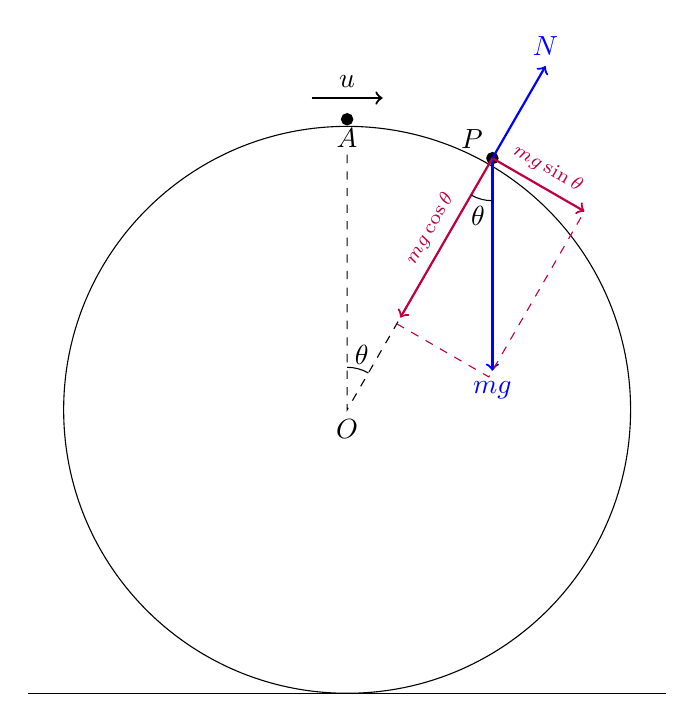
\begin{tikzpicture}[scale=0.9]
			\draw(0,0) node[below]{$O$} circle(4);
			\draw (-4.5,-4) -- (4.5,-4);
			\draw[fill] (0,4.1) circle(0.08) node[below]{$A$};
			\draw[thick,->] (-0.5,4.4) -- ++(1,0) node[midway, above]{$u$};
			\draw[fill] (60:4.1) circle(0.08) node[above left]{$P$};
			\draw[dashed] (0,3.6) -- (0,0) -- (60:4);
			\draw[blue,thick,->] (60:4.1) --++ (0,-3) node[below]{$mg$};
			\draw[purple,thick,->] (60:4.1) --++ (60:-2.598) node[midway,above,rotate=60]{{\scriptsize $mg\cos\theta$}};
			\draw[purple,thick,->] (60:4.1) --++ (-30:1.5) node[midway, above, rotate=-30]{{\scriptsize $mg\sin\theta$}};
			\draw[purple,dashed] (60:1.402) --++ (-30:1.5) --++ (60:2.598);
			\draw[blue,thick,->] (60:4.1) --++ (60:1.5) node[above]{$N$};
			\draw (60:0.6) arc(60:90:0.6);
			\node at (75:0.8) {$\theta$};
			\draw (60:3.5) arc(240:270:0.6);
			\node at (56:3.3) {$\theta$};
			\end{tikzpicture}
			
			Example \ref{ex-slidingP}
		\end{center}
	\end{minipage}
\end{figure}

from $A$ to $P$, K.E. loss = G.P.E. gain:

{\centering
	$\frac{1}{2}mu^2 - \frac{1}{2}mv^2 = mgl(1-\cos\theta)$
	
	$v^2 = u^2 - 2gl(1-\cos\theta)$
	
}

at $P$, consider the centripetal force acting:

{\centering
	$F_c = T - mg\cos\theta = \frac{mv^2}{l}$
	
	$T = mg\cos\theta + \frac{m}{l}\left(u^2 - 2gl(1-\cos\theta)\right)$
	
	$T = \frac{mu^2}{l} - mg(2 - 3\cos\theta) $
	
}

if $P$ completes full circle, string never slacks, so $T>0$ for any $\theta$

at top of circle, $\cos \theta = \cos 180^\circ = -1$, this gives minimum $T$ during the motion

{\centering
	$T_\tmin = \frac{mu^2}{l} - mg(2 + 3) > 0$
	
	$u^2 > 5gl$
	
}

minimum initial speed needed is therefore $u_\tmin = \sqrt{5gl}$ \eoe


\example{A smooth sphere of radius $R$ rests on a horizontal plane. A particle $P$ is projected horizontally with initial speed $u=\frac{1}{2}\sqrt{gR}$ from the top of the sphere and travels along the outer surface. (a) When $OP$ makes an angle $\theta$ with the upward vertical and $P$ remains in contact with the sphere, what is the normal contact force? (b) At what angle does $P$ lose contact with the sphere? (c) When the particle hits the plane, what are the horizontal and vertical components of its velocity?} \label{ex-slidingP}


from $A$ to $P$, K.E. gain = G.P.E. loss:

{\centering
$\frac{1}{2}mv^2 - \frac{1}{2}mu^2 = mgR(1-\cos\theta)$

$v^2 = u^2 + 2gR(1-\cos\theta) = \frac{1}{4}gR + 2gR(1-\cos\theta)$

$v^2 = \frac{9}{4}gR -2gR\cos\theta$

}

at $P$, consider the centripetal force acting:

{\centering
	$F_c = mg\cos\theta - N = \frac{mv^2}{R}$
	
	$N = mg\cos\theta - \frac{m}{R}\left(\frac{9}{4}gR -2gR\cos\theta\right)$
	
	$N = mg\left(3\cos\theta -\frac{9}{4}\right)$
	
}

when $P$ loses contact, contact force vanishes, i.e., $N=0$, so one has

{\centering
	$\cos\theta=\frac{3}{4} \RA \theta \approx 41.4^\circ$
	
}

after losing contact, motion only affected by gravity, so particle undergoes projectile motion

at start of projectile, the initial velocity

{\centering
	$v_0^2 = \frac{9}{4}gR - 2gR\cdot \frac{3}{4} = \frac{3}{4}gR$
	
}

horizontal component of velocity is constant, so

{\centering
	$v_x = v_{0,x} = v_0 \sin\theta \RA v_x =  \frac{\sqrt{7}}{4}\cdot \sqrt{\frac{3}{4}gR} \RA v_x = \sqrt{\frac{21gR}{64}}$
	
}

next, consider vertical motion under constant acceleration of free fall

{
	
	\centering 
	
	$v_y^2 = v_{0,y}^2 + 2gh = \left(v_0\cos\theta\right)^2 + 2g(1+\cos\theta)R = \frac{3}{4}gR\cdot \left( \frac{3}{4}\right)^2 + 2g\left(1+\frac{3}{4}\right)R \RA v_y = \sqrt{\frac{251gR}{64}} $
	
}

\example{A smooth circular hoop of radius $r$ with
	centre $O$ is fixed in a vertical plane. Two small rings $A$ and $B$, each of mass $m$, are threaded on the hoop and joined by a light inextensible string. Given that the string remains taut, $OC$ makes an angle $\theta$ with the upward vertical where $C$ is the mid-point of the string. The system is slightly displaced from its equilibrium position in
	which $\theta = 0$. At time $t$ the angle $AOB = 2\beta$. (a) By considering the total energy of the system, find an expression for the angular speed $\dot{\theta}$ of the system. (b) Find an expression for the angular acceleration $\ddot{\theta}$. (c) By considering the tangential acceleration of the rings, find the tension in the string in terms of $\theta$.} \label{ex-loopring}

\begin{figure}[htp]
	\begin{center}
		\begin{tikzpicture}[scale=1]
		\draw[thick, white, ->] (165:4) --++ (165:2.5); 
		\draw (0,0) node[below]{$O$} circle(4);
		\draw[dashed] (125:4) node[left]{$A$} -- (0,0) node[midway,below left]{$r$} -- (15:4) node[midway, below]{$r$} node[above right]{$B$};
		\draw (125:4) -- (15:4) node[midway,above]{$C$};
		\draw[dashed] (0,0) -- (70:2.294);
		\draw[very thick, rotate=125] (4,0) ellipse (0.1 and 0.05);
		\draw[very thick, rotate=15] (4,0) ellipse (0.1 and 0.05);
		\draw[dashed] (0,0) --++ (0,2);
		\draw(0,1) arc(90:70:1);
		\node at (80:1.2) {{\footnotesize $\theta$}};
		\draw(70:0.8) arc(70:15:0.8);
		\node at (42:1.1) {{\footnotesize $\beta$}};
		\draw(90:0.8) arc(90:125:0.8);
		\node at (106:1) {{\tiny $\beta-\theta$}};
		\draw[thick, blue, ->] (125:4) --++ (0,-1.8) node[left]{$mg$}; 
		\draw[thick, blue, ->] (125:4) --++ (-20:1.5) node[above]{$T$}; 
		\draw[thick, blue, ->] (125:4) --++ (125:2.5) node[above]{$N_A$}; 
		\draw[thick, blue, ->] (15:4) --++ (0,-1.8) node[left]{$mg$}; 
		\draw[thick, blue, ->] (15:4) --++ (160:1.5) node[above]{$T$}; 
		\draw[thick, blue, ->] (15:4) --++ (15:2.5) node[above]{$N_B$}; 
		\draw[dashed] (125:4) --++ (35:2);
		\draw[dashed] (125:4) --++ (215:2);
		\draw[dashed] (15:4) --++ (105:2);
		\draw[dashed] (15:4) --++ (-75:2);
		\end{tikzpicture}
		
	Example \ref{ex-loopring}
	\end{center}
\end{figure}

loss in G.P.E. for $B$ = gain in G.P.E. for $A$ + increase in K.E. for system

{

\centering

$mgr\left[\cos\beta-\cos(\beta+\theta)\right] = mgr\left[\cos(\beta-\theta) - \cos\beta\right] + 2\times\frac{1}{2}mv^2$

$v^2 = gr\left[2\cos\beta - \cos(\beta+\theta) - \cos(\beta-\theta)\right]$

}

using trigonometric identity $\cos(x\pm y) = \cos x \cos y -\mp \sin x \sin y$, we find

{

\centering

$v ^2 = gr(2\cos\beta-2\cos\beta\cos\theta) \RA v^2 = 2gr\cos\beta(1-\cos\theta)$

$\dot{\theta}^2 = \frac{v^2}{r^2} \RA \dot{\theta}^2 = \frac{2g}{r}\cos\beta(1-\cos\theta)$

}

taking time derivative of $\dot{\theta}^2$:

{

\centering

$2\dot{\theta}\cdot\ddot{\theta} = \frac{2g}{r}\cos\beta\sin\theta\cdot\dot{\theta} \RA \ddot{\theta} = \frac{g}{r}\cos\beta\sin\theta$

}

tangential motion of $A$ gives: $T\cos\beta - mg\sin(\beta-\theta) = m r\ddot{\theta}$

tangential motion of $B$ gives: $mg\sin(\beta+\theta) - T\cos\beta = m r\ddot{\theta}$

adding the two equations, one can find exactly the same result for $\ddot{\theta}$ after a bit algebra

subtracting the two equations, we obtain

{

\centering 

$2T\cos\beta = mg \sin(\beta+\theta) + mg\sin(\beta-\theta)$

}

using trigonometric identity $\sin(x\pm y) = \sin x \cos y \pm \sin x \cos y$, this simplifies to

{
	
	\centering 
	
	$2T \cos\beta = 2 mg \sin\beta \cos\theta \RA T = mg \tan\beta \cos\theta$
	
}